\documentclass[submission, LectureNotes]{SciPost}

\usepackage{amsmath, amssymb}
\usepackage{graphicx}
\usepackage{bm}
\usepackage{color}
\usepackage{enumerate}
\usepackage{physics}
\usepackage{siunitx}
\usepackage{listings}
\usepackage{pythonhighlight}
\usepackage{exercise}

\definecolor{LightGray}{rgb}{0.9, 0.9, 0.9}

\newcommand{\hatd}{{\ensuremath{\hat{d}}}}
\newcommand{\hatc}{{\ensuremath{\hat{c}}}}
\newcommand{\Ne}{{\ensuremath{N_\mathrm{e}}}}
\newcommand{\bk}{\ensuremath{{\bf k}}}
\newcommand{\br}{\ensuremath{{\bf r}}}

\newcommand{\bx}{\bm{x}}
\newcommand{\by}{\bm{y}}
\newcommand{\bS}{\bm{S}}
\newcommand{\bU}{\bm{U}}
\newcommand{\bV}{\bm{V}}
\newcommand{\bu}{\bm{u}}
\newcommand{\bv}{\bm{v}}
\newcommand{\bK}{K}
\newcommand{\brho}{\bm{\rho}}
\newcommand{\bG}{\bm{G}}
\newcommand{\wmax}{\ensuremath{{\omega_\mathrm{max}}}}
\newcommand{\Nband}{\ensuremath{{N_\mathrm{band}}}}
\newcommand\cee{\mathrm{c}}%
\newcommand\cdag{\mathrm{c}^\dagger}%
\newcommand\ee{\mathrm{e}}%
\newcommand\ii{\mathrm{i}}%
\newcommand\iv{\ii\nu}%
\newcommand\iw{\ii\omega}%
\newcommand\iW{\ii\Omega}%
\newcommand\WW{\mathcal{W}}
\newcommand\FF{\mathrm{F}}
\newcommand\BB{\mathrm{B}}
\newcommand\Fbar{\mathrm{\bar F}}
\newcommand\Bbar{\mathrm{\bar B}}
\newcommand{\GW}{{\ensuremath{GW}}}
\newcommand{\tauk}{\ensuremath{\bar{\tau}^\alpha_k}}
\newcommand{\taukF}{\ensuremath{\bar{\tau}^\mathrm{F}_k}}
\newcommand{\wk}{\ensuremath{\bar{\omega}^\alpha_k}}

\newcommand{\wkF}{\ensuremath{\bar{\omega}^\mathrm{F}_k}}

\newcommand{\hatFmat}{\hat{\mathbf{F}}}
\newcommand{\Fmat}{{\mathbf{F}}}

\newcommand{\KF}{\ensuremath{K^\mathrm{F}}}
\newcommand{\KB}{\ensuremath{K^\mathrm{B}}}
\newcommand{\kF}{\ensuremath{k^\mathrm{F}}}
\newcommand{\kB}{\ensuremath{k^\mathrm{B}}}
\def\deltaB{\delta_{\alpha, \mathrm{B}}}
\def\deltaF{\delta_{\alpha, \mathrm{F}}}

\begin{document}

\begin{center}{\Large \textbf{
    Numerical recipes for many-body physics
}}\end{center}

\begin{center}
Hiroshi Shinaoka\textsuperscript{1*},
\end{center}

\begin{center}
{\bf 1} Department of Physics, Saitama University, Saitama 338-8570, Japan
\\
* h.shinaoka@gmail.com
\end{center}

\begin{center}
\today
\end{center}


\section*{Abstract}
This lecture note reviews ....

\vspace{10pt}
\noindent\rule{\textwidth}{1pt}
\tableofcontents\thispagestyle{fancy}
\noindent\rule{\textwidth}{1pt}
\vspace{10pt}

\section{Introduction}

\clearpage
\section{Green's functions}
\subsection{Fermionic and bosonic correlation functions}
%One-particle Green's functions represent one-particle responses of an equilibrium state.
We define retarded/advanced/imaginary-time correlation functions as
\begin{align}
	G^\mathrm{R}(t-t') &= -\ii \theta(t-t')\expval{A(t)B(t')\mp B(t')A(t)},\\
	G^\mathrm{A}(t-t') &= -\ii \theta(t'-t)\expval{A(t)B(t')\mp B(t')A(t)},\\
	G(\tau-\tau') &= -\theta(\tau-\tau')\expval{A(\tau)B(\tau')} \mp \theta(\tau'-\tau) \expval{B(\tau')A(\tau)}.
\end{align}
The operators $A$ and $B$ are either fermionic or bosonic.
The signs $\mp$ are for bosons and fermions, respectively.
$\expval{\cdots}$ represents statistical average in the the grand canonical ensamble.
%The symbols $a$ and $b$ denote spin orbitals,
%while $c_a$ and $c^\dagger_b$ denote annihilation and creation operators.
%The first two are defined in real time, while the last one in imaginary time.
%
%These Green's functions 
These real-time/imaginary-time correlation functions are transformed to
real frequency and imaginary (Matsubara) frequencies, respectively:
%For a while, we focus on fermionic Green's functions.
%can be represented in a unified form using Lehmann representation:
\begin{align}
    G^\mathrm{R}(\omega) &= \int_{-\infty}^\infty \dd t e^{\ii\omega t}G^\mathrm{R}(t),\\
    G^\mathrm{A}(\omega) &= \int_{-\infty}^\infty \dd t e^{\ii\omega t}G^\mathrm{A}(t),\\
    G(\iv) &= \int_0^\beta \dd \tau e^{\iv \tau}G(\tau),\label{eq:matsubara-AB}
\end{align}
where Matsubara frequencies are given by $\nu = 2n\pi/\beta$ and $\nu = (2n+1)\pi/\beta$ for bosons/fermions, respectively ($n\in \mathbb{Z}$).
We defined $\beta = 1/T$ ($k_\mathrm{B}=1$).
%These correlation functions be analytically transformed to each other as we will see later.

In the grand canonical ensemble, $G(\iv)$ has the Lehmann representation:
\begin{align}
    G_{AB}(\iv) &= \int \dd \omega \frac{\rho_{AB}(\omega)}{\iv - \omega},\\
    \rho_{AB}(\omega) &\equiv -\frac{1}{\pi} \imaginary G_{AB}(\omega + 0^+)\\
    & = \frac{1}{Z}\sum_{mn}(e^{-\beta E_n} \mp e^{-\beta E_m})
    \mel{n}{A}{m}\mel{m}{B}{n}
    \delta(\omega - (E_m-E_n)),\label{eq:matsubara-lehmann}
\end{align}
where
$n$, $m$ run over all eigenstates of the system ($E_{m/n}$ denotes an eigenvalue).
%We introduced the extra factor $\omega^{\delta_{\alpha,\mathrm{B}}}$ for bosons ($\alpha$ represents the staistics),
%whose reasoning will be explained later.

Using Eq.~\eqref{eq:matsubara-lehmann},
we can analytically continue $G(\iv)$ to the whole complex plane as $G(z)$ for $z\in \mathbb{C}$.
Note that there are poles or a branch cut on the real axis.
%Using $G_{AB}(z)$, the real-frequency and imaginary-frequency (Matsubara) Green's funcitons are analytically continued as
The advanced and retarded Green's functions are given by the value of $G_{AB}(z)$ above/below the real axis as
\begin{align}
    G^\mathrm{R}_{AB}(\omega) &= G_{AB}(\omega+\ii 0^+),\\
    G^\mathrm{A}_{AB}(\omega) &= G_{AB}(\omega+\ii 0^-).
\end{align}
Due to the branch cut on the real axis, $G^\mathrm{R}_{AB}(\omega) \neq G^\mathrm{A}_{AB}(\omega)$ in general.

At high frequencies, $G(\iv)$ decays in power.
Applying partial integration recursively to Eq.~\eqref{eq:matsubara-AB},
we obtain its high frequency expansion,
\begin{align}
    G_{AB}(\iv) &= 
    \frac{c^{(1)}_{AB}}{\iv} +
    \frac{c^{(2)}_{AB}}{(\iv)^2} +
    \frac{c^{(3)}_{AB}}{(\iv)^3} + \cdots,
\end{align}
where
\begin{align}
    c^{(m)}_{AB} &= (-1)^{m} \qty(G_{AB}^{(m-1)}(0^+) - G_{AB}^{(m-1)}(0^-)).
\end{align}
In particular, one can show
\begin{align}
   c^{(1)}_{AB} &= \poissonbracket{A}{B}.
\end{align}

\subsection{Imaginary-time representation}
\textcolor{red}{Write it!}

\subsection{Fermionic one-particle Green's function}
We focus on the fermionic cases where $A$ and $B$ are annihilation and creation operators of fermions, respectively.
In such cases, the correlation is called ``(one-particle) Green's function''.
The Lehmann representation of the Green's function reads
\begin{align}
    G_{ab}(\iv) &= \int \dd \omega \frac{\rho_{ab}(\omega)}{\iv - \omega},\\
    \rho_{AB}(\omega) &\equiv -\frac{1}{\pi} \imaginary G_{ab}(\omega + 0^+)\\
    & = \frac{1}{Z}\sum_{mn}(e^{-\beta E_n} + e^{-\beta E_m})
    \mel{n}{c^\dagger_a}{m}\mel{m}{c_b}{n}
    \delta(\omega - (E_m-E_n)),\label{eq:matsubara-g-lehmann}
\end{align}
where $a$ and $b$ denote spin orbitals.

Applying partial integration recursively to Eq.~\eqref{eq:matsubara-AB},
we obtain a high frequency expansion of the Green's function,
\begin{align}
    G_{ab}(\iv) &= 
    \frac{c^{(1)}_{ab}}{\iv} +
    \frac{c^{(2)}_{ab}}{(\iv)^2} +
    \frac{c^{(3)}_{ab}}{(\iv)^3} +
    O\qty(\frac{1}{(\iv)^4}),
\end{align}
where
\begin{align}
    c^{m}_{ab} &= (-1)^{m} \qty(G_{ab}^{(m-1)}(0^+) - G_{ab}^{(m-1)}(0^-)).
\end{align}
In particular, one can show
\begin{align}
   c^{0}_{ab} &= \poissonbracket{c_a}{c^\dagger_b} = \delta_{ab}.
\end{align}

This clearly indicates that the Green's function has a discontinuity at $\tau=0,\pm \beta, \pm 2\beta$ for $a=b$.
At these points, the off-diagonal components ($a\neq b$) have a slope discontinuity or a discontinuity in higher-order derivatives.
For $0 <\tau < \beta$, the Green's function is a smooth and analytic function.
%
%The sum rules is followed by $c_{ab}^1 = \delta_{ab}$.
%The slow power-law decay originates from the discontinuity of $G(\tau)$ and its derivatives at $\tau=0,\pm \beta, \pm 2\beta, \cdots$.
%\
%
%Below, we summarize the analytic properties of the fermionic Green's function.
%
%Pros:
%\begin{itemize}
    %\item $G(\tau)$ is a smooth function for $0<\tau<\beta$.
    %\item Good resoluation at low frequencies
%\end{itemize}
%
%Cons:
%\begin{itemize}
    %\item $G(\tau)$ is not continuous at $\tau=0,\pm \beta, \cdots$, leading to the nesscecity of cumbersome numerical tricks.
    %\item Numerical analytic continuation to high frequencies is not stable.
%\end{itemize}

\subsection{Example: Hubbard atom}
We consider the single-orbital fermionic Hubbard atom at half filling:
\begin{align}
   \mathcal{H} &= U n_\uparrow n_\downarrow - \mu (n_\uparrow + n_\downarrow),
\end{align}
where $\mu= U/2$ and $U>0$.
By simple calculations, one obtains
\begin{align}
    G_{\sigma\sigma'}(z) &= \frac{1}{2}\qty(\frac{1}{z-U/2} + \frac{1}{z+U/2})\delta_{\sigma\sigma'},\label{eq:gz-hubbard-atom}
\end{align}
where $\sigma$ and $\sigma'$ are spin indices.
This can be transformed to the imaginary-time domain as
\begin{align}
    G_{\sigma\sigma'}(\tau) &= -\frac{1}{2}
    \qty(
        \frac{e^{-\tau U/2}}{1+e^{-\beta U/2}} +
        \frac{e^{\tau U/2}}{1+e^{\beta U/2}}
    )\delta_{\sigma\sigma'}\label{eq:gtau-hubbard-atom}
\end{align}
for $0 < \tau<\beta$.

%\subsection{Exercise 1}
\begin{Exercise}[label=ex1]
Plot Eqs.~\eqref{eq:gz-hubbard-atom} and \eqref{eq:gtau-hubbard-atom} for a typical value of $\beta$.
You will see that $G(\tau)$ changes very rapidly around $\tau=0$ and $\beta$ at large $\beta$.
Due to the sum rule and the half-filling condition,
$G_{\sigma\sigma'}(0^+)=G_{\sigma\sigma'}(\beta+0^-) = -1/2$.
On the other hand, $G(\iv)$ decays only algebraically at high frequencies.
Your plot should look like Figs.~\ref{fig:gtau-hubbard-atom} and~\ref{fig:giv-hubbard-atom}.
\end{Exercise}

\begin{figure}
    \centering
    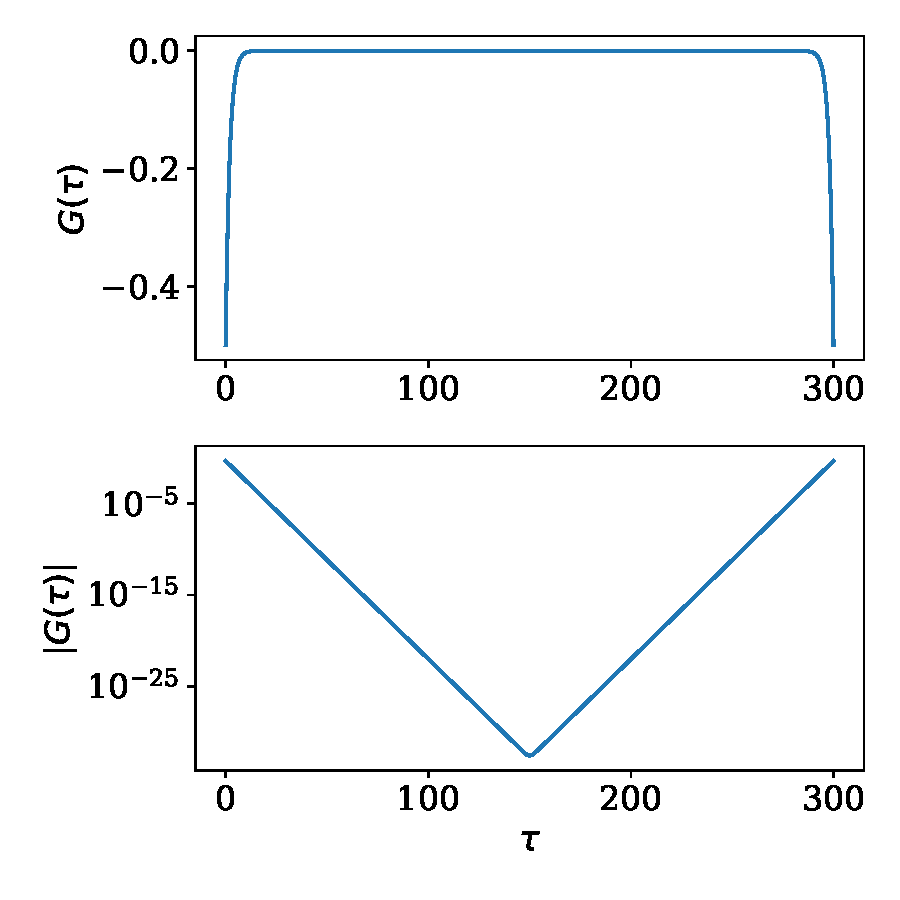
\includegraphics[width=0.5\columnwidth]{gtau_hubbard_atom.pdf}
    \caption{$G(\tau)$ computed for the Hubbard atom with $U=1$ and $\beta=300$.}
    \label{fig:gtau-hubbard-atom}
\end{figure}
\begin{figure}
    \centering
    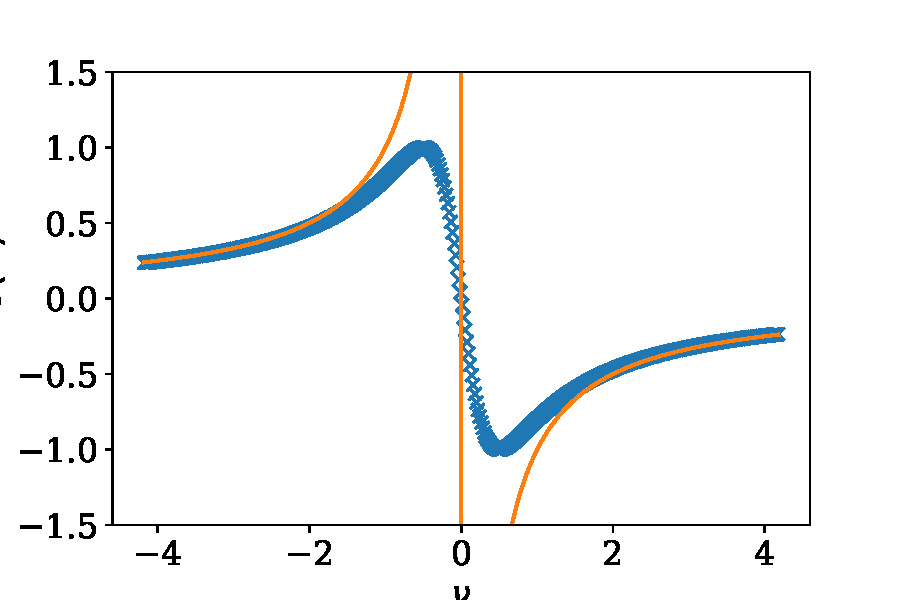
\includegraphics[width=0.5\columnwidth]{giv_hubbard_atom.pdf}
    \caption{$G(\iv)$ computed for the Hubbard atom with $U=1$ and $\beta=300$. The solid curve denotes $-1/\nu$.}
    \label{fig:giv-hubbard-atom}
\end{figure}

\begin{Exercise}
Derive Eq.~\eqref{eq:gtau-hubbard-atom} from Eq.~\eqref{eq:gz-hubbard-atom} using 
the formula
\begin{align}
   T\sum_{\nu} \frac{e^{-\iv\tau}}{\iv - \epsilon} &= - \frac{e^{-\epsilon\tau}}{1+e^{-\beta\epsilon}}.\label{eq:single-pole-ft}
\end{align}
\end{Exercise}

\begin{Exercise}[label=ex:native-inverse-transform]
Please numerically check how $G(\tau)$ of the Hubbard atom behaves near $\tau=0$ if we truncate the summation in Eq.~\eqref{eq:single-pole-ft} at some frequency.
The result should look like Fig.~\ref{fig:naive-inverse-transform-hubbard-atom}.
\end{Exercise}

\begin{figure}
    \centering
    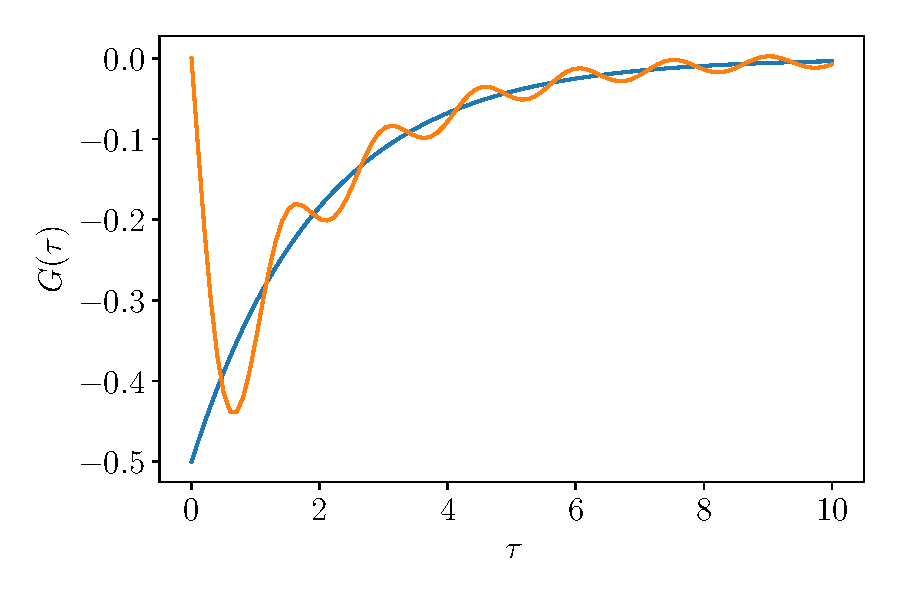
\includegraphics[width=0.5\columnwidth]{naive_inverse_transform_hubbard_atom.pdf}
    \caption{Naive inverse transform of $G(\iv)$ for the Hubbard atom with $U=1$ and $\beta=300$. We used 200 positive Matsubara frequencies.}
    \label{fig:naive-inverse-transform-hubbard-atom}
\end{figure}


\clearpage
\section{Conventional approaches}
\subsection{Uniform mesh}
Due to the algebraic decay of $G(\iv)$ and the strong $\tau$ dependence of $G(\tau)$ around $\tau=0$,
it is a bit cumbersome to treat the Green's function numerically.
In this section, we explain a conventional way of doing so.

A naive way to store the values of the Green's function numerically is to use uniform meshes in $\iv$ and $\tau$.
Although you will see that this fails at low temperatures later,
it may be instructive to start with the simplest one.
In the imaginary-frequency domain, we use a uniform mesh consisting of the lowest $2N_\nu$ imaginary frequencies:
\begin{align}
&\qty{(2n+1)\pi/\beta~| n=-N_\nu, -N_\nu+1, \cdots N_\nu-2, N_\nu-1}.
\end{align}
In the imaginary-time domain, we use a uniform mesh,
\begin{align}
&\qty{\frac{\beta t}{N_\tau-1}~|~t=0, 1, \cdots, N_\tau-1},
\end{align}
where the two end points are interpreted as $0^+$ and $\beta + 0^-$.

Let us consider to discretize a $G(\tau)$ on the uniform mesh as $G_t$ ($t=0, \cdots, N_\tau-1$).
How many mesh points are sufficient for representing $G(\tau)$ accurately?
We consider the simplest case, i.e. the Hubbard atom Eq.~\eqref{eq:gtau-hubbard-atom}.
In this case, $G(\tau)$ can be approximated around $\tau=0$ as
\begin{align}
    G(\tau) &\propto e^{-\tau U/2}.
\end{align}
This indicates that we must increase the density of the mesh points proportionally with $U$ around $\tau=0$.
Considering the band width of the spectrum is $U$, one can see that $N_\tau$ must increase as $O(\beta \wmax)$ in general cases,
where $\wmax$ is a cutoff frequency of the spectrum: i.e., the spectrum is non-zero only in $[-\wmax, \wmax]$.

\subsection{Interpolation}
Even if $G(\tau)$ is known only on a discrete set of data points,
we may want to evaluate it on arbitrary points.
This can be done by interpolating $G(\tau)$ for $0 < \tau < \beta$.
Popular choices are linear interpolation and cubic spline interpolation.
The linear interpolation fits the data using linear piecewise polynomials
and construct new data points within the range of the known data points.
The cubic spline interpolation uses piecewise polynomials of degree 3.
We demonstrate them for the Hubbard atom in Fig.~\ref{fig:interpolation-gtau}.
One can see that the cubic spline interpolation yields better results.
At an arbitrary point, the interpolation error generally vanishes as $O(h^2)$ and $O(h^4)$
for the linear and cubic spline interpolation methods, respectively,
where $h\equiv \beta/N$ and $N$ is the number of data points.

\begin{Exercise}
    Confirm numerically the scaling of the interpolation error 
    with respect to $h$ for these two interpolation methods.
\end{Exercise}

\begin{figure}
    \centering
    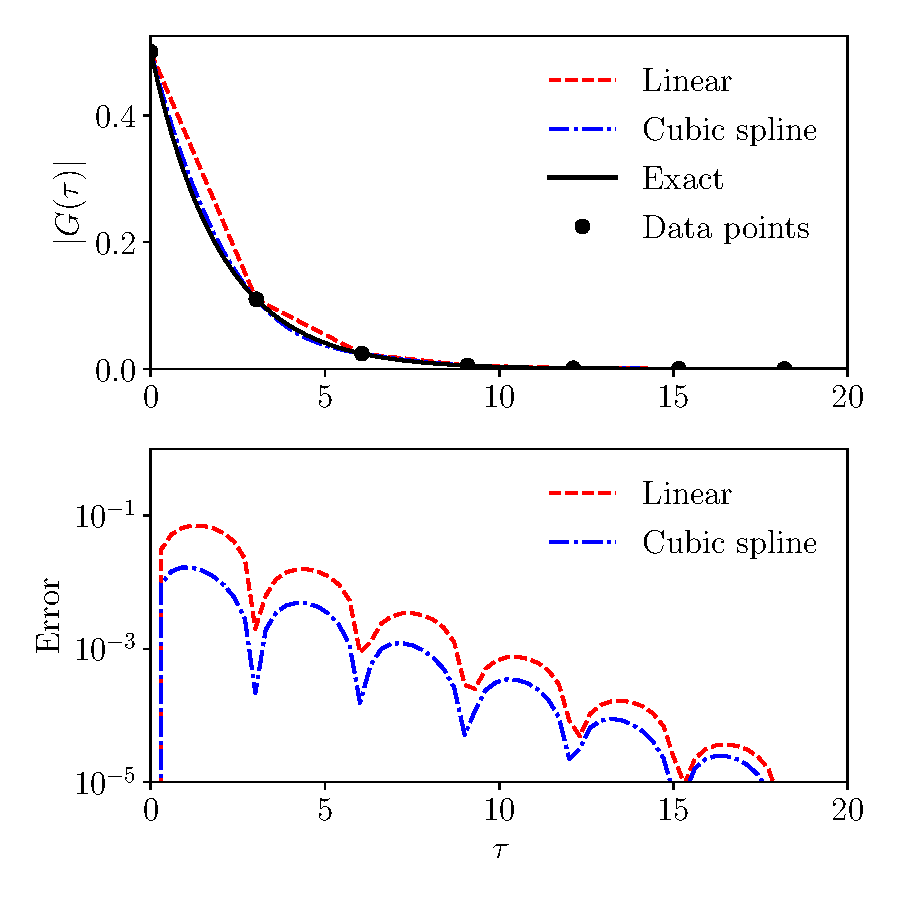
\includegraphics[width=0.8\columnwidth]{interpolation_gtau.pdf}
    \caption{
        Linear and cubic spline interpolations of $G(\iv)$ for the Hubbard atom with $U=1$ and $\beta=300$.
        We used 100 data points.
        }
    \label{fig:interpolation-gtau}
\end{figure}

%
%Thus, we need to \textit{interpolate} the values to evaluate the Green's function in between mesh points.
%An easy way is to use some piecewise polynomial interpolation.
%This is justified by the fact that $G(\tau)$ is a smooth function for $0< \tau<\beta$.

\subsection{Fourier transform}
We explain a naive way to transform numerical data on a uniform mesh in $\tau$ to Matsubara frequencies.
%First, we introduce a quadrature rule for approximating the definite integral of a function.
First, we introduce quadrature rules.
A quadrature rule approximates the definite integral over interval $[-1,1]$ as
\begin{align}
   \int_{-1}^1 f(x) dx \simeq \sum_{i=1}^n w_i f(x_i),
\end{align}
where $w_i$ is a positive weight and $x_i$ is a node.
Different quadrature rules use different choices of weights and nodes.
A popular choice is Gaussian quadrature, which yields accurate results if $f(x)$ can be approximated 
well by a polynomial of degree $2n-1$ or less.

Using your favorite quadrature rule (and interpolation if necessary),
one can Fourier transform numerical data of $G(\tau)$ as
\begin{align}
   G(\iv) &\approx \sum_{i=1}^{n} \tilde{w}_i e^{\iv \tau_i} G(\tau_i),\label{eq:naive-fourier-transform}
\end{align}
where $\tau_i = (x_i+1)\beta/2$ and $\tilde{w}_i=(\beta/2) w_i$.
The RHS of Eq.~\eqref{eq:naive-fourier-transform} converges to the exact value in the limit of $n \rightarrow \infty$.

Figure~\ref{fig:fourier-transform-hubbard-atom} show a numerical demonstration of the Fourier transform using Gauss quadrature.
One can see that the numerical error is very small at low frequencies but the error goes up above some frequency cutoff.

\begin{Exercise}
    Explain why the procedure fails at high frequencies and 
    figure out what determines the cutoff frequency.
    How can we improve on it? (Hint: see Section~\ref{sec:inverse-fourier-transform}).
\end{Exercise}

\begin{figure}
    \centering
    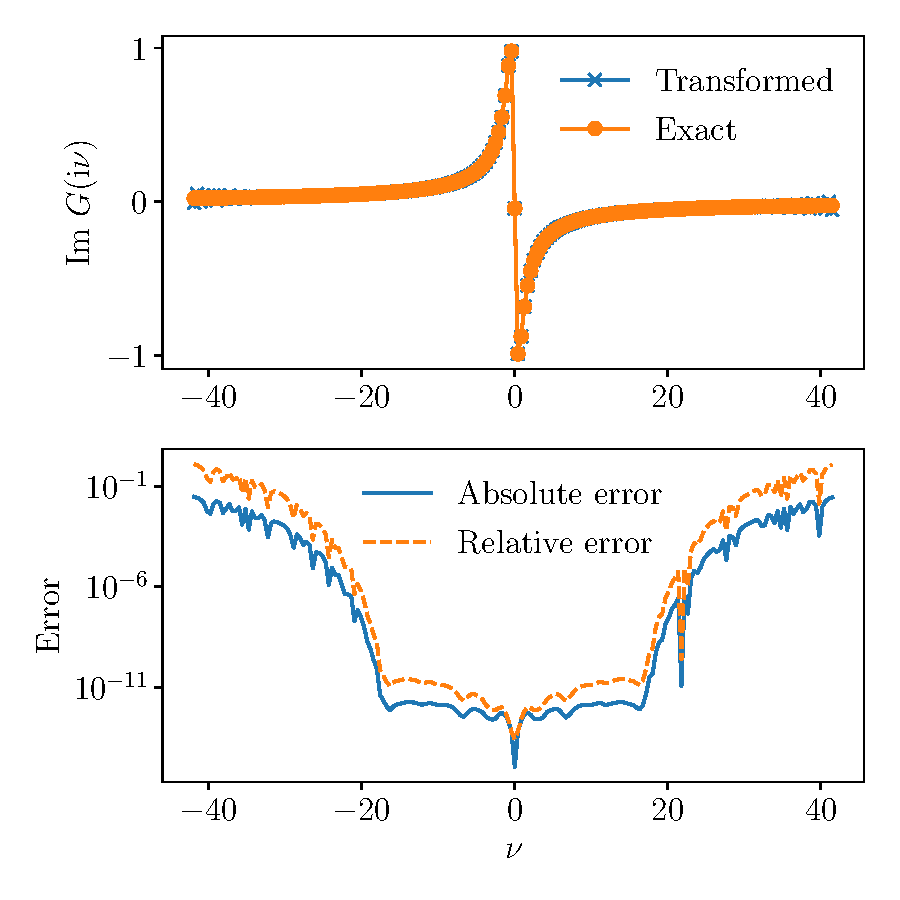
\includegraphics[width=0.8\columnwidth]{fourier_transform_hubbard_atom.pdf}
    \caption{
        Fourier transformation from $G(\tau)$ to $G(\iv)$ for the Hubbard atom with $U=1$ and $\beta=300$.
        We used Gauss quadrature with $n=1000$.
        }
    \label{fig:fourier-transform-hubbard-atom}
\end{figure}

%We first interpolate the numerical value of $G(\tau)$ on a finer mesh in $\tau$, e.g., by using cubic spline interpolation.
%Then, we compute
%\begin{align}
   %G(\iv) &\approx \frac{\beta}{N_{\tau'}}\sum_{t=0}^{N_{\tau'}-1} e^{\iv \tau_t} G_t,\label{eq:naive-fourier-transform}
%\end{align}
%where $\tau_t = \frac{\beta t}{N_{\tau'}-1}$ and $G_t$ is the interpolated value at a grid point and $N_{\tau'} > 2 N_\tau$.

\subsection{Inverse Fourier transform}\label{sec:inverse-fourier-transform}
Another tricky thing is inverse Fourier transform of $G(\iv)$ to $G(\tau)$.
As we have already seen in Exercise~\ref{ex:native-inverse-transform},
the naive inverse Fourier transform does not work at all.
In this subsection, we explain a simple procedure to avoid this problem.
If the first moment of the high-frequency expansion is exactly known,
we can subtract the first term of the expansion from $G(\iv)$ as
\begin{align}
    \tilde{G}(\iv) &\equiv G(\iv) - \frac{c^0}{\iv}.
\end{align}
A native inverse Fourier transformation of $\tilde{G}(\iv)$ is safer than that of $G(\iv)$ because 
$\tilde{G}(\iv)$ has only a slope discontinuity in the $\tau$ domain.
For $0 < \tau<\beta$,
\begin{align}
    G(\tau) &\approx \sum_{n=-n_\mathrm{max}}^{n_\mathrm{max}} e^{\ii \nu_n \tau }\tilde{G}(\iv) - \frac{c^0}{2},\label{eq:inverse-transform-c0}
\end{align}
where $\nu_n = (2n+1)\pi/\beta$.
The inverse Fourier transforms of higher-order terms can be found in Appendix B of the E. Gull's Ph. D thesis.

The computation complexity of the naive implementation of Eq.~\eqref{eq:inverse-transform-c0} scales as $O(N_\tau n_\mathrm{max})$.
This can be greatly reduced to $O(N\log N)$ for $N=N_\tau \propto n_\mathrm{max}$ by using fast Fourier transform.
However, we do not describe it because the sparse sampling approach is far more efficient anyway.

\begin{Exercise}
    Implement Eq.~\eqref{eq:inverse-transform-c0} for the Hubbard atom and confirm that the discontinuity at $\tau=0$ is correctly reproduced.
\end{Exercise}


\clearpage
\section{Legendre basis}
\subsection{Definition}
L. Boehnke and co-workers proposed a more compact representation of the Matsubara/imaginary-time Green's functions, the so-called Legendre basis~\cite{Boehnke:2011dd}.
They proposed to expand $G(\tau)$ for $0<\tau<\beta$ as
\begin{align}
    G(\tau) &= \sum_{l=0}^\infty \frac{\sqrt{2l+1}}{\beta} P_l(x(\tau)) G_l,\label{eq:legendre-gtau}\\
    G_l &= \sqrt{2l+1} \int_0^\beta d\tau P_l(x(\tau)) G(\tau),
\end{align}
where $x(\tau) = 2\tau/\beta -1$ and $G_l$ are expansion coefficients.
Because $G(\tau)$ is a smooth function for $0 < \tau < \beta$, the expansion coefficients $G_l$ generally decay exponentially.

$P_n(x)$ is a polynomial of degree $n$.
Legendre polynomials form an orthogonal system with respect to weight function 1 over the interval $[-1,1]$.
The Legendre polynomials satisfy the orthogonality condition
\begin{align}
    \int d x P_m(x) P_l(x) = \frac{2}{2n+1} \delta_{mn},
\end{align}
and the recursion formula
\begin{align}
    (n+1)P_{n+1}(x) &= (2n+1) x P_n(x) - n P_{n-1}(x).
\end{align}
The recursion formula can be used to evaluate the Legendre polynomials at given $x$.
The first few Legendre polynomials are 
\begin{align}
    P_0(x) &= 1,\\
    P_1(x) &= x,\\
    P_2(x) &= \frac{1}{2}(3x^2-1).
\end{align}
\begin{figure}[h]
    \centering
    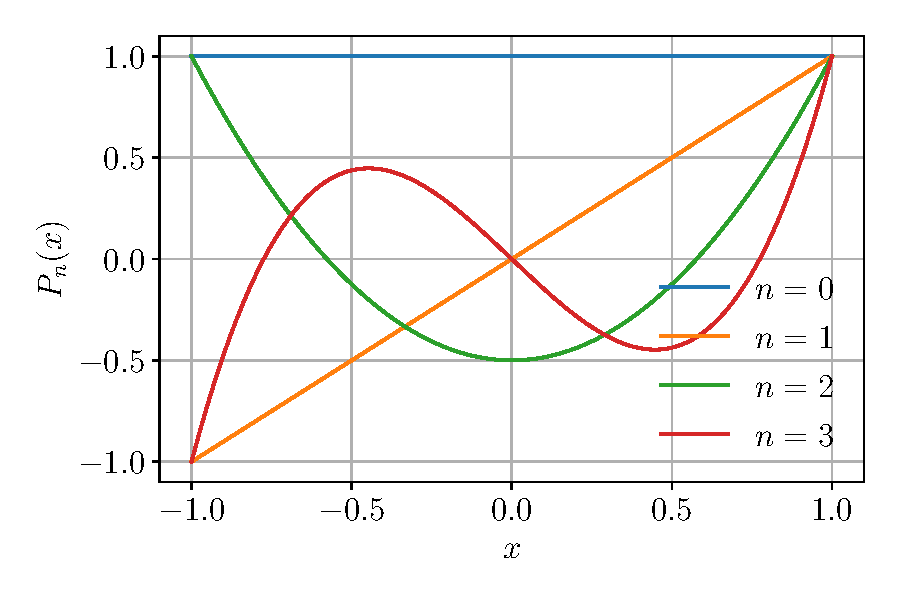
\includegraphics[width=0.6\columnwidth]{legendre_polynomials.pdf}
    \caption{Legendre polynomials}
    \label{fig:legendre_polynomials}
\end{figure}

$P_n(x)$ has exactly distinct $n$ roots $\{x_{\nu n}\}$ ($\nu=1,\cdots,n$) in the interval $[-1,1]$.
The properties of the roots (zeros) have been investigated extensively in the literature.
One nice property is 
\begin{align}
    \frac{\nu-1/4}{n+1/2} \pi < \theta_{\nu n} < \frac{\nu}{n+1}\pi
\end{align}
for $1 \le \nu \le n/2$ and $x_{\nu n} = \cos \theta_{\nu n}$~\cite{Szego.1936.Szego}.
Thus, the position of the root closest to 1, which coressponds to $\tau=\beta$, scales as
\begin{align}
    1-x_{1 n} &\approx \frac{1}{2}\theta_{1 n}^2 \propto 1/n^2
\end{align}
for $n\rightarrow +\infty$.
We now assume that $G(\tau)$ decays as $G(\tau) \propto e^{-W\tau}$.
To resolve this feature in the expansion using the Legendre basis,
the number of basis functions must satisfy $N \propto \sqrt{\beta}$.
A more detailed discussion is found in Appendix B of Ref.~\cite{Chikano:2018gd}.
%P. Nevai, Orthogonal polynomials, Mem. Amer. Math. Soc. 213 (1979).

The Fourier transform of Eq.~\eqref{eq:legendre-gtau} is given by
\begin{align}
    G(\iv) &= \sum_{l=0}^\infty T_{nl} G_l,
\end{align}
where
\begin{align}
    T_{nl} &\equiv \frac{\sqrt{2l+1}}{\beta} \int_0^\beta d\tau e^{\iv \tau} P_l(x(\tau))\nonumber\\
    &= (-1)^n \ii^{l+1} \sqrt{2l+1}j_l(m\pi/2),
\end{align}
with $j_l(z)$ denoting the spherical Bessel functions and $\nu = m \pi/\beta$.
Bosonic/fermionic Matsubara frequencies are denoted by even/odd $m$.

\subsection{Numerical examples}
We now demonstrate the accuracy of the Legendre basis for the same model (Hubbard atom, $\beta=300$).


\begin{figure}
    \centering
    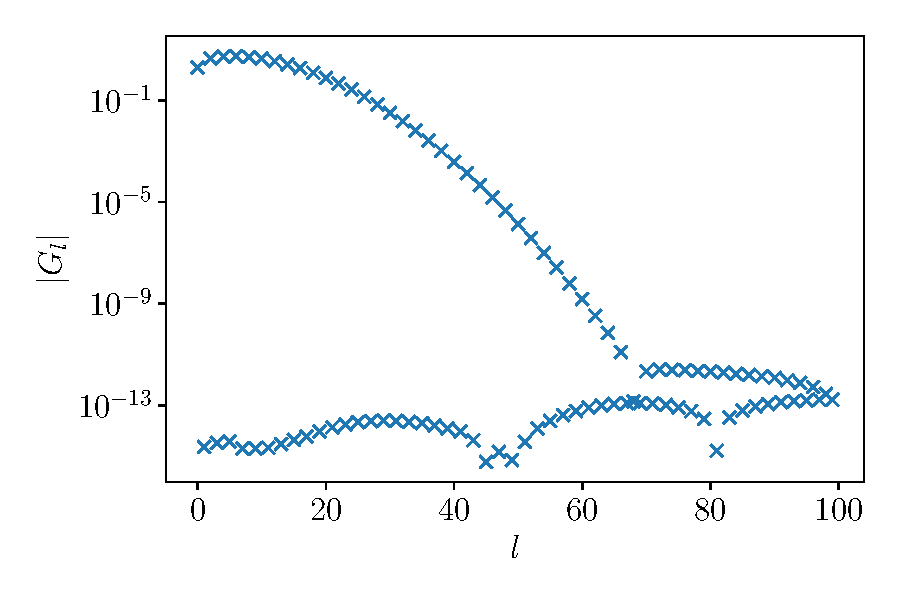
\includegraphics[width=0.8\columnwidth]{legendre_hubbard_atom.pdf}
    \caption{
        Expansion coefficients in the Legendre basis computed
        for the Hubbard atom with $U=1$ and $\beta=300$.
        }
    \label{fig:legendre-hubbard-atom}
\end{figure}

\begin{figure}
    \centering
    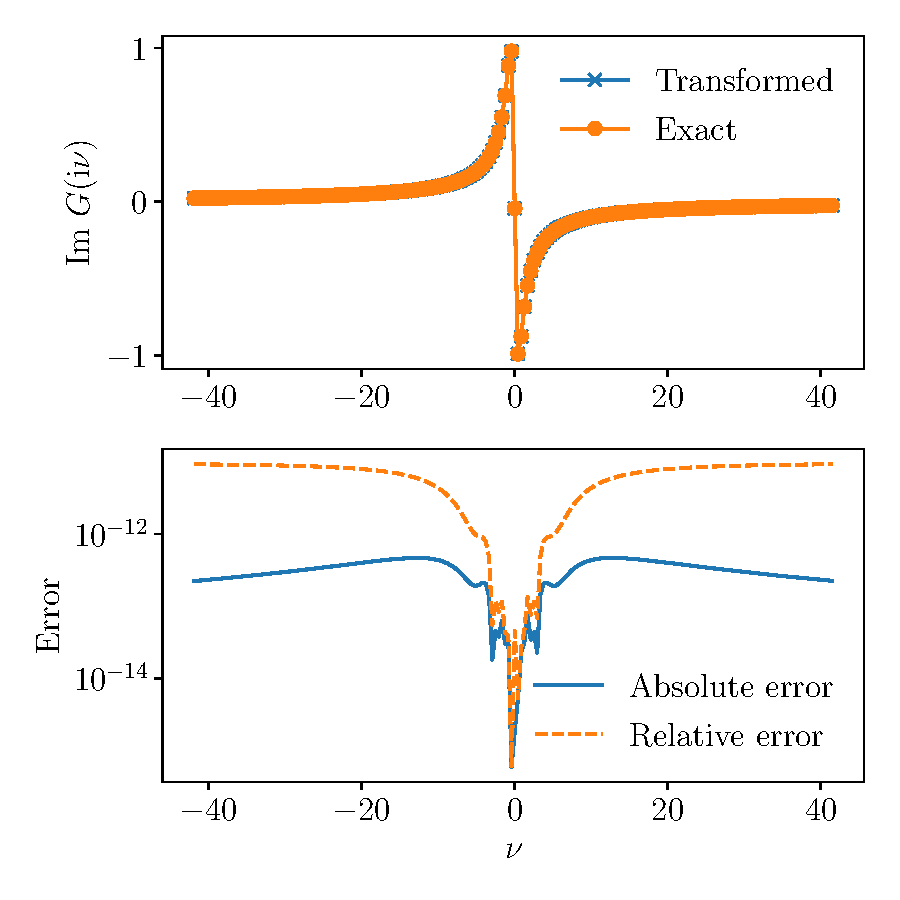
\includegraphics[width=0.8\columnwidth]{legendre_matsu_hubbard_atom.pdf}
    \caption{
        $G(\iv)$ reconstructed from the expansion coefficients in the Legendre basis
        for the Hubbard atom with $U=1$ and $\beta=300$ (see Fig.~\ref{fig:legendre-hubbard-atom}).
        }
    \label{fig:legendre-matsu-hubbard-atom}
\end{figure}


\begin{Exercise}
    Compute expansion coefficients of the Green's function of the Hubbard atom
    for lower temperatures.
    Check how the number of basis functions scales with respect to $beta$.
\end{Exercise}



\clearpage
\section{Why are imaginary-time data highly compressible?}
%We refer the reader to Ref.~\cite{shinaoka2021efficient} for the technical details of
%the IR basis and the sparse sampling method.
%Before going into technical details, we intuitevly show 
In this section, we show that numerical data of imaginary Green's funcitons are highly compressible.
As shown in Eq.~\eqref{eq:matsubara-lehmann},
the Green's function $G(\tau)$ is related with the corresponding spectral function.
In many numerical calcualtions, what we compute is the imaginary-time Green's function $G(\tau)$.
But, we want to ``reconstruct'' the corresponding spectral function from the numerical data of $G(\tau)$.
Can we simply invert the integral equation in Eq~\eqref{eq:matsubara-lehmann}?
No, we cannot.
This is a well-known infamous ill-posed inverse problem.

To illustrate this problem, we show two spectral functions in Fig.~\ref{fig:three_gaussian}.
The original spectral function consists of three Gaussian peaks,
while the second one denoted by the broken line is slighly broaden and is not even non-negative.

We now transform these spectral functions to $\tau$ using
\begin{align}
    G(\tau) &= - \int_{-\omega_\mathrm{max}}^{\omega_\mathrm{max}}d\tau K^\mathrm{F}(\tau, \omega) \rho(\omega),\label{eq:anacont-f}
\end{align}
where
$$
K^\mathrm{F}(\tau, \omega) = \frac{e^{-\tau\omega}}{1+e^{-\beta\omega}}.
$$
We compare the obtain results in Fig.~\ref{fig:three_gaussian_gtau}.
Although the two spectral functions are significantly different, 
the two Green's functions agree within an accuracy of $10^{-5}$.
Why is $G(\tau)$ insensitive to changes in $\rho(\omega)$?
This originates from some special properites of the kernel.

We now discretize the kernel using uniform meshes
($[-\omega_\mathrm{max}, \omega_\mathrm{max}]$ and $[0,\beta]$) as
\begin{align}
   (\bK)_{ij} &\equiv \frac{2\wmax}{N_\omega}K(\tau_i, \omega_j).
\end{align}
We set the number of mesh points to $N_\omega = N_\tau=1000$.
Then, we perform the SVD of the obtained matrix $\boldsymbol{K}$ as
\begin{align}
    \boldsymbol{K} &= \boldsymbol{U} \boldsymbol{S} \boldsymbol{V}^\dagger,
\end{align}
where $\boldsymbol{U}$ and $\boldsymbol{V}$ are matrices consisting of singular vectors
and $\boldsymbol{S}$ is a diagonal matrix consisting of the correpsonding singular values $s_i$ ($\ge 0$).
Figure~\ref{fig:kf-singular-vals} plots the largest 30 singular values computed for $\wmax=10$ and $\beta=10$.

We denote the column vectors of $\bU$ and $\bV$ associated with the singular value $s_i$
by $\bu_i$ and $\bv_i$ ($i=1,2,\cdots$).
Then, Eq.~\eqref{eq:anacont-f} can be transformed into
\begin{align}
    g_i = - s_i \rho_i,
\end{align}
where
\begin{align}
    g_i    &= u_i^\dagger \bm{g},\\
    \rho_i &= v_i^\dagger \bm{\rho}.
\end{align}
Here, $\bm{g}$ and $\bm{\rho}$ are the column vectors consisting of the values of $G(\tau)$ and $\rho(\omega)$ on the mesh points.

Figure~\ref{fig:gi_rhoi} shows the two spectral functions and the associated $G(\tau)$ projected on the singular vectors.
Now you can see that the ``reconstructed'' spectral function agree with the original one up to $i=12$.
Although $\rho_i$ does not decay exponentially (due to the finite-size effects of $N_\omega$),
$g_i$ decay exponentially due to the singular values.
This is why $G(\tau)$ associated with the ``reconstructed'' spectral function
matches the original one well.

\begin{figure}
    \centering
    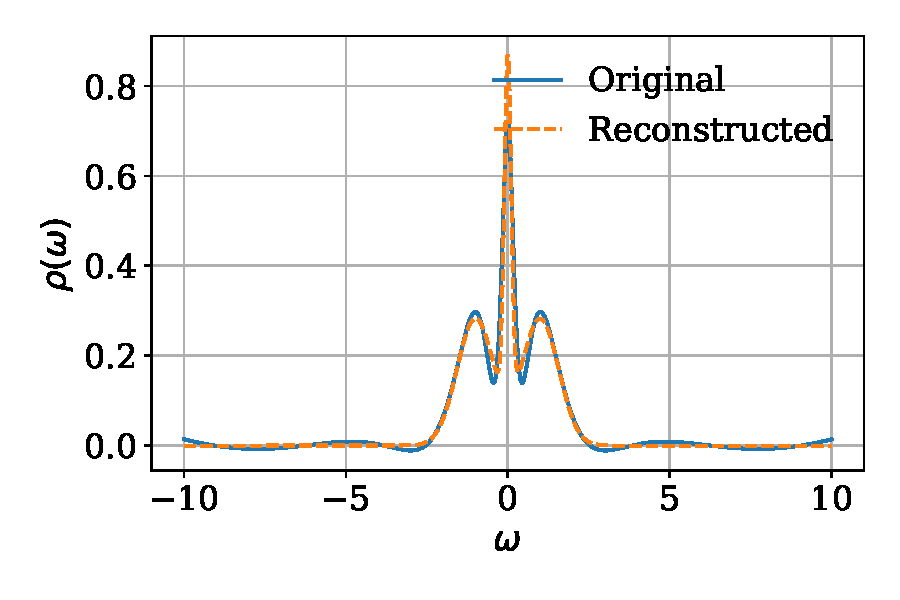
\includegraphics[width=0.6\columnwidth]{three_gaussian.pdf}
    \caption{
      Spectral functions consisting of three Gaussian peaks.
      The solid line denotes the original spectral function.
      The broken line denotes the reconstructed one by analytic continuation (see the text).
    }
    \label{fig:three_gaussian}
\end{figure}

\begin{figure}
    \centering
    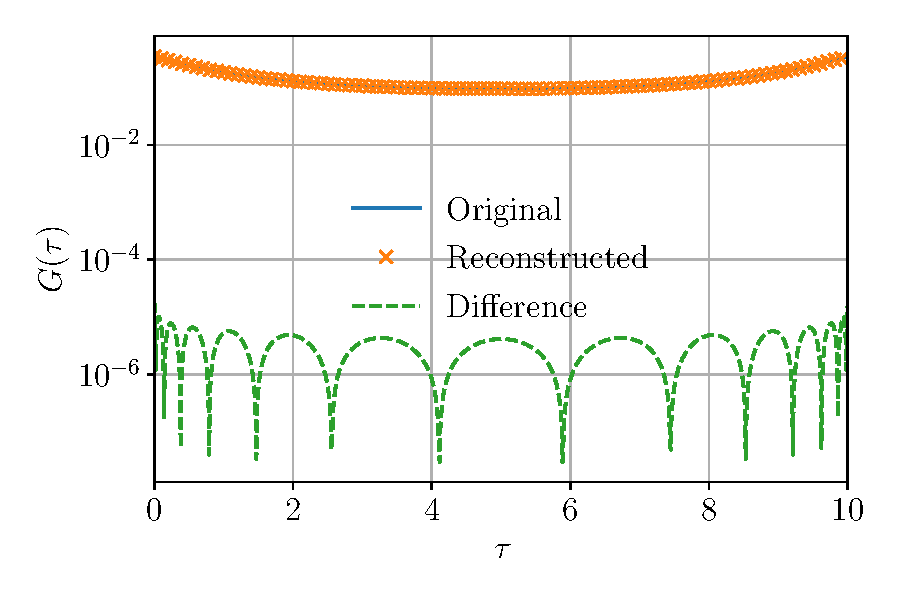
\includegraphics[width=0.6\columnwidth]{three_gaussian_gtau.pdf}
    \caption{
      Green's functions transformed from the two spectral functions in Fig.~\ref{fig:three_gaussian}
      for $\beta=10$.
      }
    \label{fig:three_gaussian_gtau}
\end{figure}

\begin{figure}
    \centering
    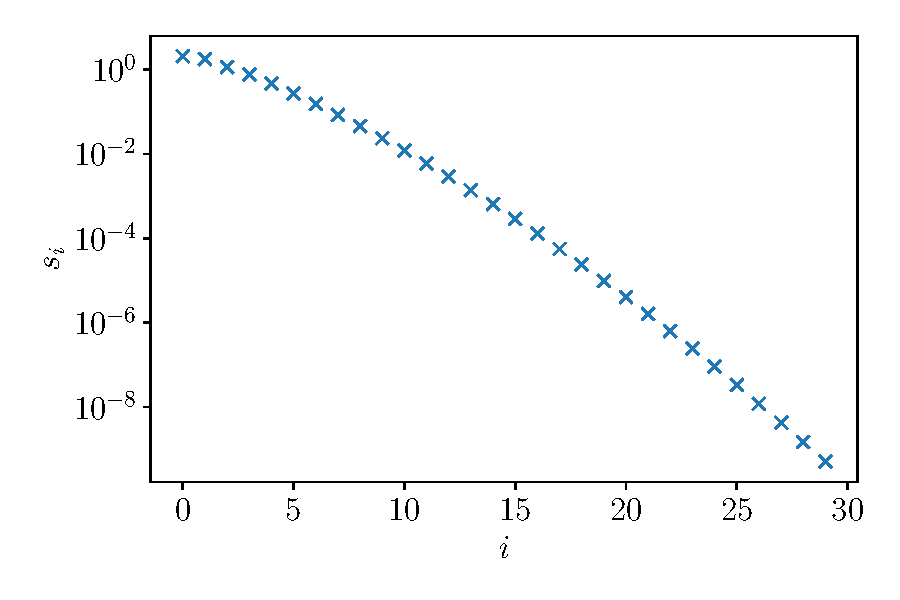
\includegraphics[width=0.6\columnwidth]{kf_singular_vals.pdf}
    \caption{
    Singular values of the fermionic kernel discretized using $N_\omega=N_\tau=1000$ for $\wmax=\beta=10$.
    We plot only the first 30 singular values.
    }
    \label{fig:kf-singular-vals}
\end{figure}

\begin{figure}
    \centering
    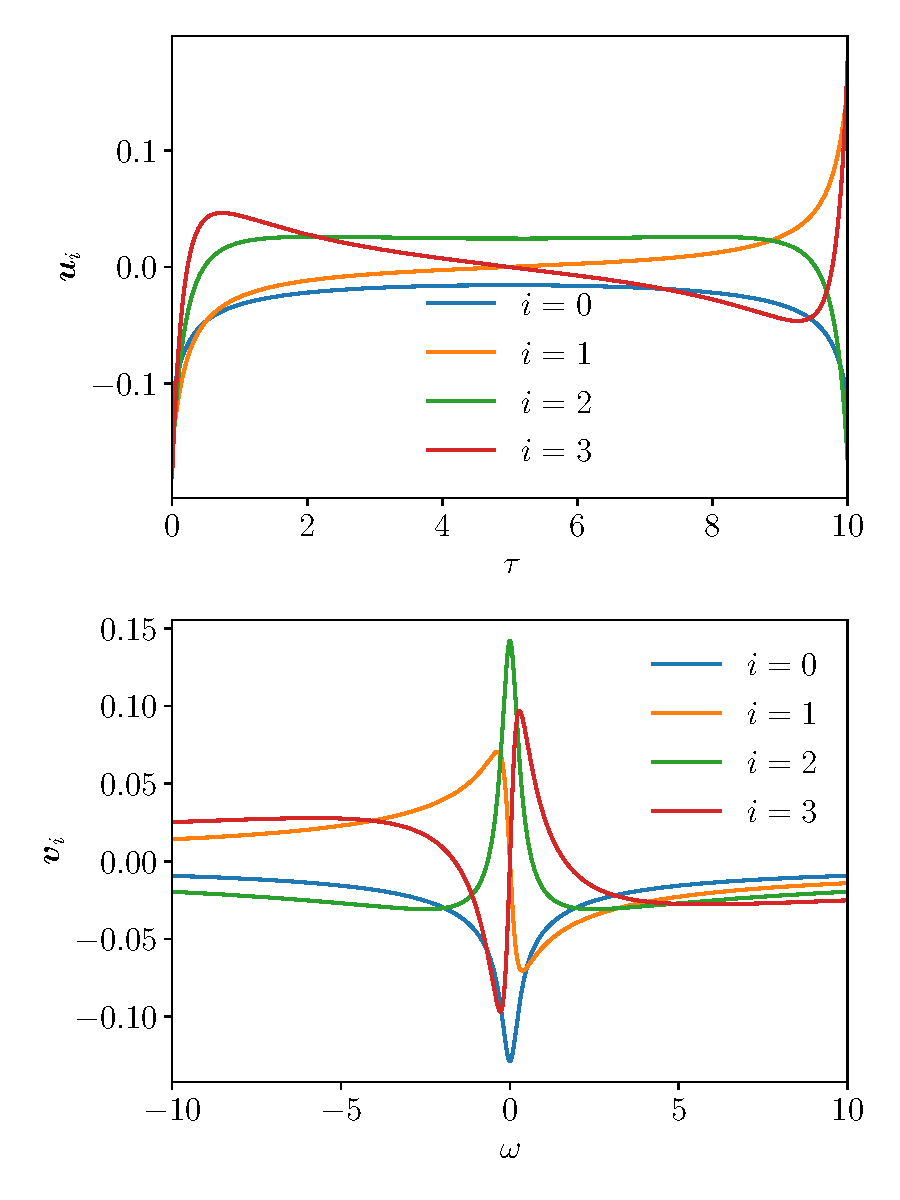
\includegraphics[width=0.6\columnwidth]{kf_singular_vectors.pdf}
    \caption{
        Singular vectors associated with the singular values in Fig.~\ref{fig:kf-singular-vals}.
    }
    \label{fig:kf-singular-vectors}
\end{figure}

\begin{figure}
    \centering
    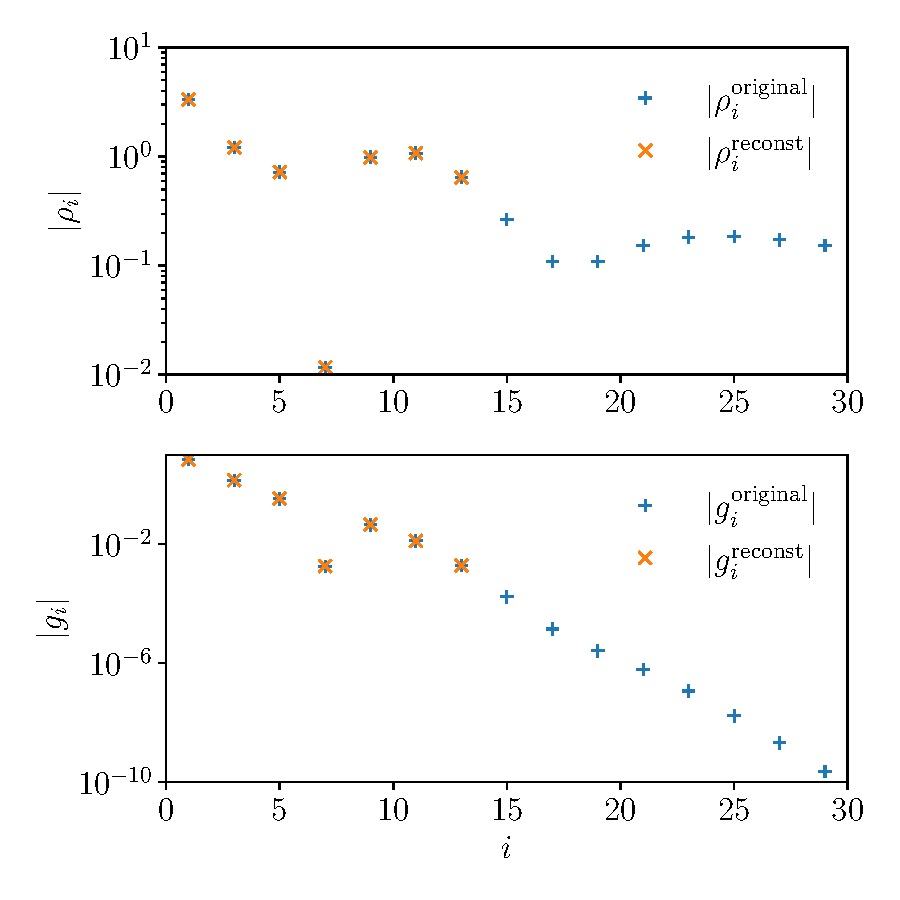
\includegraphics[width=0.6\columnwidth]{gi_rhoi.pdf}
    \caption{
      Two spectral functions in Fig.~\ref{fig:three_gaussian}
      and the associated Green's functions projected onto the singular vectors.
      }
    \label{fig:gi_rhoi}
\end{figure}



\begin{Exercise}
    Genearate another spectural function by taking more singular vectors.
    What happens if we take too many singular vectors?
\end{Exercise}


\clearpage


%In this section, we provide only supplementary information on these technologies that is not reviewed in the lecture note.
%We use the same notation as used in the lecture.

\section{Intermediate representation (IR)}
%The bosonic IR basis is defined in terms of the SVD of the bosonic kernel
We now sophisticate the ideas of the SVD presented in the previous section.
\subsection{Fermionic case}
In the imaginary-time domain, the Lehmann represenation reads 
\begin{align}
    G(\tau) &= - \int_{-\wmax}^\wmax \dd\omega \KF(\tau, \omega) \rho(\omega),\label{eq:gtau-fermion}
\end{align}
where 
\begin{align}
    \KF(\tau, \omega) &= \frac{e^{-\omega\tau}}{1 + e^{-\beta\omega}}.
\end{align}
The so-called intermediate representation (IR) basis functions are defined in terms of singular value expansion as
\begin{equation}
    K^\mathrm{F}(\tau,\omega)=
    \sum_{l=0}^\infty U_l(\tau)S_l V_l(\omega)\label{eq:sve-tau}
\end{equation}
for a fixed frequency cutoff $\wmax$.
The IR basis functions and singular values are the solution of the integral equation
\begin{align}
    S_l U_l(\tau) &= \int_{-\wmax}^\wmax \dd\omega \KF(\tau, \omega) V_l(\omega).\label{eq:integral-eq}
\end{align}
In practice, one can solve this integral equation by projecting the equation onto some basis sets for $\tau$ and $\omega$
such as piecewise Legendre polynomials~\cite{Chikano:2018gd}.
The user however does not have to implement a solver
because a well-tested Python implementation is available~\cite{irbasis2019,irbasis3}.
As summarized in Ref.~\cite{shinaoka2021efficient}, the IR basis functions have the following properites:
\begin{description}
    \item[Property 1] The singular values $S_l$ are non-degenerate, non-negative, and monotonically decrease faster than exponentially with respect to $l$.
    \item[Property 2] The number of numerically significant singular values (e.g., $S_l/S_0 \ge 10^{-15}$) is determined by the dimensionless quantity $\Lambda\equiv\beta\wmax$ and increases only logarithmically with respect to $\Lambda$.
    \item[Property 3] $U_l(\tau)$ and $V_l(\omega)$ can be chosen to be real functions, and they then become even-odd functions for even-odd $l$. In this convention, $\hat{U}_l^\alpha(\iw)$ is purely imaginary or real.
    \item[Property 4] $U_l(\tau)$ and $V_l(\omega)$ have $l$ roots. In addition, in the limit of $\beta\wmax\rightarrow 0$ (a high-temperature limit), $U_l^\alpha(\tau(x))$ and $V_l^\alpha(\omega(x))$ coincide with the Legendre polynomial $P_l(x)$ up to a constant [$\tau(x) \equiv \beta(x+1)/2$, $\omega(x) \equiv x \wmax$ for $-1 < x < 1$].
\end{description}

\subsection{Bosonic case}
%We consider a bosonic correlation function
%\begin{equation}
    %\hat{G}(\iw)=\int_0^\beta\dd{\tau}\ee^{\iw\tau}\langle T_{\tau}A(\tau)B(0)\rangle,\label{eq:giwdef}
%\end{equation}
%where $A$ and $B$ are bosonic operators.
%Its Lehmann representation function reads
%\begin{equation}
    %\hat{G}(\iw)=\int_{-\wmax}^\wmax\dd{\omega'} K^\mathrm{B}(\iw,\omega')\rho(\omega'),
%\end{equation}
%where the bosonic kernel is defined by
In the original proposal of the IR basis~\cite{Shinaoka:2017ix,Chikano:2018gd},
they proposed to use different basis functions for bosons.
In this lecture, as proposed in a recent follow-up paper~\cite{kaye2021discrete},
we use the same basis functions for bosons as those for fermions.

For a bosonic correlation function, the Lehmann representation in $\tau$ reads
\begin{align}
    G(\tau) &= - \int_{-\wmax}^\wmax \dd \omega \frac{e^{-\omega\tau}}{1-e^{-\beta\omega}} \rho(\omega)\nonumber\\
    &= -  \int_{-\wmax}^\wmax \dd\omega \KF(\tau, \omega) \tilde \rho(\omega),\label{eq:gtau-boson}
\end{align}
where $\rho(\omega) = - \frac{1}{\pi}\imaginary G(\omega+\ii 0^+)$ and we defined an auxiliary spectral function
\begin{align}
    \tilde \rho(\omega) &\equiv \frac{1+e^{-\beta\omega}}{1-e^{-\beta \omega}} \rho(\omega).
\end{align}
From Eq.~\eqref{eq:matsubara-lehmann}, one can show that the spectral function has a general form of
\begin{align}
   \rho(\omega) &= \rho_0\beta\epsilon \delta(\omega - \epsilon) + \rho_1(\omega),\label{eq:rho-split}
\end{align}
where $\rho_1(\omega)$ is a smooth function linearly vanishing at $\omega=0$ and $\epsilon$ is an infinitesimal number.
%If any, the delta function comes from zero-energy exciations.
%At low frequencies, we obtain
%\begin{align}
   %\rho(\omega) &= \rho_0 \delta(\omega) + \rho_1 \omega
%\end{align}
%If any, the delta function commes from zero-energy exciations.
%Thus, 
%At low frequencies, we obtain
Then, the auxiliary spectral function reads
\begin{align}
   \tilde \rho(\omega) &\simeq \left(\frac{2\rho_0\epsilon}{\omega}\right) \delta(\omega-\epsilon) + \frac{2\rho_1(\omega)}{\beta\omega},\label{eq:trho-split}
\end{align}
where the second term is a smooth function around $\omega=0$.
Substituting Eq.~\eqref{eq:trho-split} into Eq.~\eqref{eq:gtau-boson} yields
\begin{align}
    G(\tau) &= -\rho_0 - \int_{-\wmax}^\wmax \dd\omega \KF(\tau, \omega) \tilde \rho_1(\omega),\label{eq:gtau-boson-split}
\end{align}
where $\tilde \rho_1(\omega) \equiv \frac{1+e^{-\beta\omega}}{1-e^{-\beta\omega}} \rho_1(\omega)$.
Because $\tilde \rho_1(\omega)$ is a smooth and non-divergent function, one can use the fermionic IR basis funcitons
to expand the non-singular part of the bosonic correlation function.
The singular term, i.e., the constant term in $\tau$, must be treated separately if any.

%\subsection{Dimensionless representation}
%\textcolor{red}{Write it!}

\subsection{Numerical demonstration}
We now demonstrate how to generate IR basis functions by decomposing the kernel using the Python library
\texttt{irbasis3}.
This can be used in the Julia language through \texttt{PyCall.jl}.
You can install \texttt{irbasis3} by running the following command from a shell:
\begin{verbatim}
$ pip install -U irbasis3 xprec
\end{verbatim}
Alternatively, you can use a template jupyter notebook at Google Colab~\cite{colab-template}.
In the repository, we provide two Jupyter notebooks (section6.ipynb, section6\_julia.ipynb)
for Python and Julia, where we
\begin{enumerate}
    \item define a kernel object,
    \item generate IR basis using singular value expansion,
    \item plot singular values/basis functions.
\end{enumerate}

%\subsubsection{Basis object}
In Python, we can generate a feromioc basis object \texttt{basis}
by computing singular values down to $S_l/S_0 \simeq 10^{-10}$
for $\Lambda=10^2$ and $\beta=10$ as follows:
\begin{python}
import irbasis3
lambda_ = 100
beta = 10
K = irbasis3.KernelFFlat(lambda_=100)
basis = irbasis3.FiniteTempBasis(K, statistics='F', beta=beta, eps=1e-10)
\end{python}

%\subsubsection{Singular values}
The data attribute \texttt{s} of the basis object
stores all the available singular values:
\begin{python}
 basis.s
\end{python}

\begin{python}
array([1.45387261e+00, 1.24137141e+00, 7.98387159e-01, 5.34115485e-01,
3.19202855e-01, 1.88195405e-01, 1.06269952e-01, 5.84664007e-02,
3.12626140e-02, 1.62959998e-02, 8.28608690e-03, 4.11383766e-03,
1.99543191e-03, 9.46115126e-04, 4.38678206e-04, 1.98971153e-04,
8.83076718e-05, 3.83596425e-05, 1.63120097e-05, 6.79164595e-06,
2.76915058e-06, 1.10582146e-06, 4.32562293e-07, 1.65764896e-07,
6.22400190e-08, 2.28998146e-08, 8.25716208e-09, 2.91821977e-09,
1.01098806e-09, 3.43374895e-10])
\end{python}

%\subsubsection{Basis functions}
The data attributes \texttt{u} \texttt{v} of the basis object are
\texttt{PiecewiseLegendrePoly} objects representing IR basis functions
for $\tau$ and $\omega$, respectively.
You can evaluate the basis functions as follows:
\begin{python}
basis.u(np.array([0, 0.5*beta, beta]))
\end{python}
You can learn how to use them in the notebook.

\begin{figure}
    \centering
    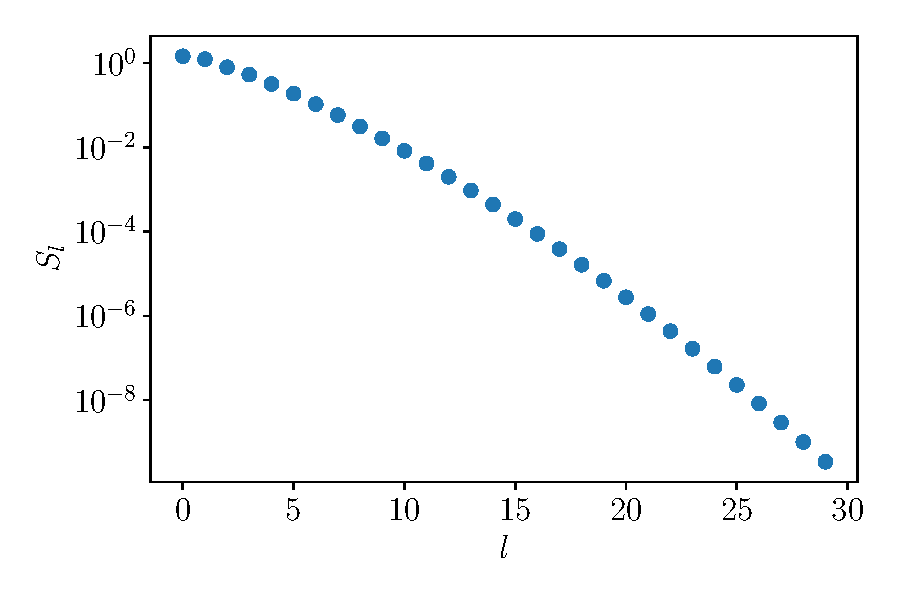
\includegraphics[width=0.6\columnwidth]{ir_basis_svals.pdf}
    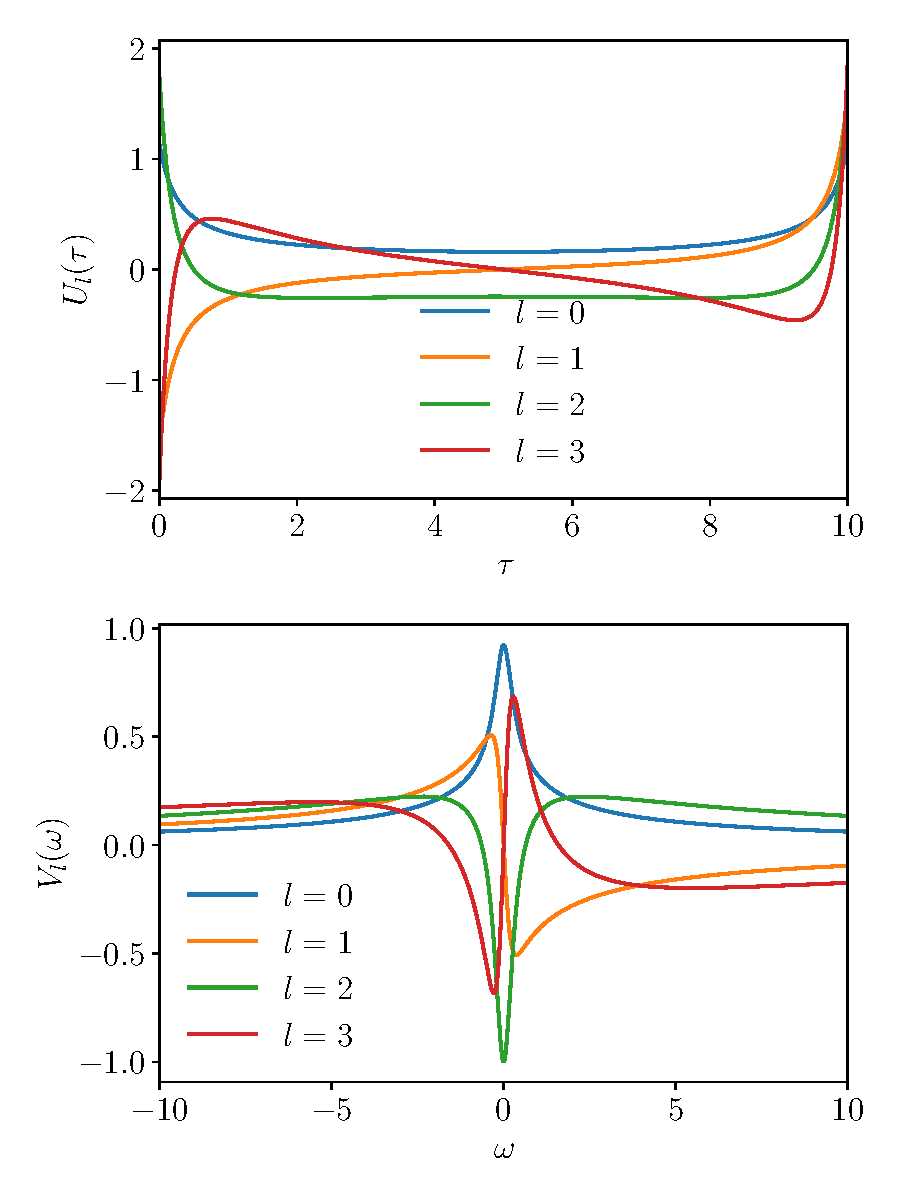
\includegraphics[width=0.6\columnwidth]{ir_basis_functions.pdf}
    \caption{
        Singular values and IR basis functions computed by \texttt{irbasis3} for $\Lambda=100$ and $\beta=10$.
    }
    \label{fig:irbasis}
\end{figure}

%An instance of \texttt{FiniteTempBasis} has many data attributes and functions,
%which we summarize in Table~\ref{table:finite_temp_basis}.
%\begin{table}[ht]
    %\centering
    %\begin{tabular}{ccc}
        %Attribute name & Type       & Description \\
        %S              & 1D ndarray & Singular values \\
        %u              &            & IR basis functions for $\tau$\\
        %%v              &            & IR basis functions for $\omega$
    %\end{tabular}
    %\caption{}
    %\label{table:finite_temp_basis}
%\end{table}

\begin{Exercise}
    Expand your favorite spectral function in $V_l(\omega)$ and compute the expansion coefficients
    of $G(\tau)$ using the relation $G_l = -S_l \rho_l$.
    Then, evaluate $G(\tau)$ on a uniform mesh.
    Note that $\rho(\omega) = \delta(\omega-\omega_0)$ yields $\rho_l = V_l(\omega_0)$.
\end{Exercise}

%\begin{Exercise}
%\end{Exercise}
%
%\begin{python}
%import numpy as np
%\end{python}


%\begin{align}
    %K^\mathrm{B}(\iw, \omega') &= \frac{\omega'}{\iw-\omega'}.\label{eq:KB-matsu}
%\end{align}
%The spectral function is defined by
%\begin{equation}
    %\rho(\omega) = -\frac{\omega}{\pi}
    %\mathrm{Im} \hat G(\omega+\mathrm{i}0^+).
        %\label{eq:rho}
%\end{equation}
%The bosonic kernel is transformed to the $\tau$ space as
%\begin{align}
    %K^\mathrm{B}(\tau,\omega') &= \frac{\omega' e^{-\tau\omega'}}{1-e^{-\beta\omega'}}.\label{eq:KB-tau}
%\end{align}
%The extra factor of $\omega'$ in Eq.~\eqref{eq:KB-matsu} was inroduced
%to avoid the divengence of $K^\mathrm{B}(\tau,\omega')$ in the limit of $\omega'\rightarrow 0$.
%In Eq.~\eqref{eq:KB-matsu}, the two $\omega'$ in the numerator and denominator cancel out in this limit.
%
%The IR basis functions, i.e., singular functions of the kernel, are illusrated in Fig.~\ref{fig:uvB}.
%%\begin{equation}
    %\hat{G}^\alpha(\iw)=\int_0^\beta\dd{\tau}\ee^{\iw\tau}\langle T_{\tau}A^\alpha(\tau)B^\alpha(0)\rangle,\label{eq:giwdef}
%%\end{equation}
%As discussed in Ref.~\ref{Chikano:2018gd}, the IR basis functions are insulating.


%As an example, let us look at the density-density correlation function of the Hubbard atom.
%This correlation function includes a constant term in $\tau$, which corresponds to a delta function at zero frequency.
%
%\begin{itemize}
    %\item Zero frequency peak
%\end{itemize}

\clearpage
\section{Transforming numerical data}
In this section,
we explain how to transform data between real-frequency/Matsubara-frequency/IR-basis domains.

\subsection{From real frequency to IR basis}
It is straightforwad to compute expansion coefficients in the IR 
from a given spectral function.
This can be done by evaluating the integral
\begin{align}
    \rho_l &= \int_{-\wmax}^\wmax \dd \omega V_l(\omega) \rho(\omega).
\end{align}

As seen in the previous section,
the distribution of $V_l(\omega)$ is much denser than Legendre polynomial $P_l(x(\tau))$ around $\tau=0, \beta$.
Thus, evaluating the integral precisely requires the use of composite Gauss–Legendre quadrature,
where the whole inteval $[-\wmax, \wmax]$ is divided to subintervals and the normal Gauss-Legendre quadrature is 
applied to each interval.
The roots of $V_l(\omega)$ for the highest $l$ used in the expansion
is a reasonable choice of the division points.
If $\rho(\omega)$ is smooth enough within each subinterval,
the result converges exponentially with increasing the degree of the Gauss-Legendre quadrature.

We demonstrate how to do this transform using \texttt{irbasis3} for the spectral function consisting 
of three Gausssian peaks (see the solid line of Fig.~\ref{fig:three_gaussian}).
This can be done by using the \texttt{overlap} function associated with the basis object \texttt{basis}
as follows:
\begin{python}
gaussian = lambda x, mu, sigma:\
    np.exp(-((x-mu)/sigma)**2)/(np.sqrt(np.pi)*sigma)

rho = lambda omega: 0.2*gaussian(omega, 0.0, 0.15) + \
    0.4*gaussian(omega, 1.0, 0.8) + 0.4*gaussian(omega, -1.0, 0.8
rhol = basis.v.overlap(rho)
\end{python}
Here, \texttt{rho} is a function that evaluates the values of the spectral function at given real frequencies.
We internally use the Gauss-Legendre quadrature for the numerical integration.
The result \texttt{rhol} is a 1D array containing $\rho_l$.
For the full source code, see section7.ipynb.


\subsection{From imaginary-time domain to IR basis}
\subsubsection{Numerical integration}
A numerically stable way to compute the expansion coefficients of $G(\tau)$ in the IR basis
is evaluating the integral
\begin{align}
    G_l &= \int_0^\beta \dd \tau G(\tau) U_l(\tau).
\end{align}

This can be done again by using composite Gauss-Legendre quadrature
based on the roots of $U_l(\tau)$ for the larget $l$ used in the expansion.
This requires to evaluate $G(\tau)$ on quadrature nodes whose number is roughly 
$N P$ ($N$ is the size of the IR basis and $P$ is the degeree of the quadrature).
From experience, $P=10$--$20$ are large enough.
At low tempertures,
this number scales logarithmically with $\beta$.
%This functionality is implemented in \texttt{irbasis3}, which can be used as follows:
This can be done similarly to the case of $\rho(\omega)$ as follows:
\begin{python}
gl_reconst = basis.u.overlap(eval_gtau)
\end{python}
Here, \texttt{eval\_gtau} is a function that evaluates the values of $G(\tau)$ at given imaginary times.
%We internally use the Gauss-Legendre quadrature for the numerical integration.
The result \texttt{gl\_reconst} is a 1D array containing the computed $g_l$.
For the full source code, see section7.ipynb.

\subsubsection{Sparse sampling}
The expansion coefficients can be evaluated by using even a fewer sampling points in the imaginary-time domain.
This is achieved by using sparse-sampling techniques.
The essential idea is simple.
If we want to determine $N$ coefficients $G_l$,
we need to know $G(\tau)$ on only up to $N$ sampling points.
Let $\bar{\tau}_1 < \cdots < \bar{\tau}_N$ be such sampling points,
one can evaluate the expansion coefficients as
\begin{align}
    g_l &= \underset{g_l}{\mathrm{argmin}}
        \sum_k \bigg| \hat G(\tauk) - \sum_{l=0}^{L-1} \hat U_l(\tauk)G_l \bigg|^2\nonumber \\
    &= \pqty{\Fmat^+ \boldsymbol{g}}_l,\label{eq:fittau}
\end{align}
where we define $(\Fmat)_{kl} = U_l(\tauk)$ and $\Fmat^+$ is its pseudo inverse.
%In practice, different choices of sampling points lead to different numeri
The numerical stability of this ``fitting'' scheme is determined
by the condition number of the coefficient matrix $\Fmat$.
An empiritically good our choice is to use the middle points of the neighboring roots of 
$U_{N-1}(\tau)$ (see Fig.~\ref{fig:sampling_points_tau}).
\begin{figure}
    \centering
    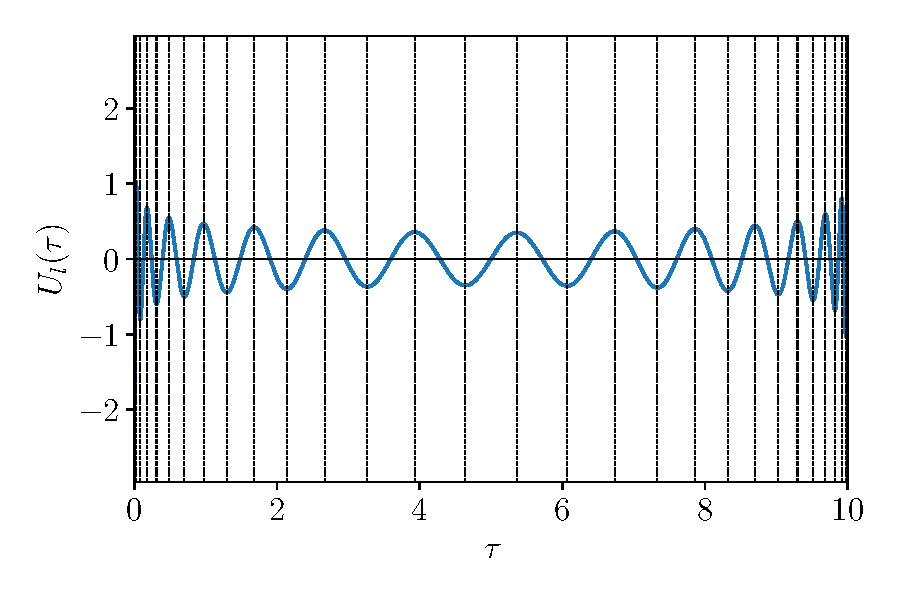
\includegraphics[width=0.6\columnwidth]{sampling_points_tau.pdf}
    \caption{
    Basis function $U_l(\tau)$ with $l=29$ computed for $\wmax=10$ and $\beta=10$.
    The vertical lines are the associated sampling points.
    }
    \label{fig:sampling_points_tau}
\end{figure}
The generation of sampling points and fitting can be done as follows:
\begin{python}
smpl = irbasis3.TauSampling(basis)
print("Sampling points: ", smpl.sampling_points)
print("Condition number: ", smpl.cond)
gl_reconst_sparse = smpl.fit(eval_gtau(smpl.sampling_points))
\end{python}
Here, \texttt{eval\_gtau} is a function that evaluates $G(\tau)$ at given imaginary times.
For $\wmax=\beta=10$ and $N=30$, the condition number is as small as 5.89.

\subsection{From Matsubara-frequency domain to IR basis}
\subsubsection{Dense mesh}

\subsubsection{Sparse sampling}

\subsection{Robustness against noise and regularization}

As reviewed in the lecture note, \textit{fitting} is a convenient way to transform numerical data either in the imaginary-time domain or in the imaginary-frequency domain.
In the practical calculations, we need a special care on the numerical stability of the fitting.
We explain how to do it in a stable way using several typical cases.

%\subsubsection{Fitting \textit{clean} numerical data}
\begin{itemize}
    \item Matsubaqra data
    \item Regularization
    \item Condition number
    \item What if the data is not \textit{clean}?
    \item How to detect overfitting
\end{itemize}

\clearpage
\section{Second-order perturbation}

\clearpage
\section{Random phase approximation}
\subsection{Hartree-Fock approximation}
\clearpage
\subsection{Restricted Hartree-Fock calculations of sigle-orbital Hubbard model}

\clearpage
\subsection{Unrestricted Hartree-Fock calculations of multi-orbital Hubbard model}
In this subsection, we briefly reivew the unrestricted Hartree-Fock approximation of multi-obital Hubbard model.
We consider a multi-orbital Hubbard model:
\begin{align}
    \hat{H} &= \sum_{ij=1}^N t_{ij} \hat{c}^\dagger_i \hat{c}_j + \frac{1}{2} \sum_{ijkl=1}^N U_{ijlk}\hat{c}^\dagger_i \hat{c}^\dagger_j \hat{c}_k \hat{c}_l
\end{align}
Here, we \textit{assume} the following properties:
\begin{align}
U_{iilk} &= 0,\label{eq:U-prop-start}\\
U_{ijll} &= 0,\\
U_{ijlk} &= U_{jikl}, \\
U_{ijlk} &= U_{lkij}^*.\label{eq:U-prop-end}
\end{align}

The antisymmetrized Colomb matrix elements are defined by
\begin{align}
    \bar{U}_{ijlk} &\equiv U_{ijlk} - U_{ijkl}.
\end{align}
These satisfy
\begin{align}
\bar{U}_{ijlk} &= -\bar{U}_{ijkl} = -\bar{U}_{jilk}
\end{align}
in addition to Eqs.~(\ref{eq:U-prop-start})--(\ref{eq:U-prop-end}).
In this notation, the Hamiltonian reads
\begin{align}
    \hat{H} &= \sum_{ij=1}^N t_{ij} \hat{c}^\dagger_i \hat{c}_j + \frac{1}{4} \sum_{ijkl=1}^N \bar{U}_{ijlk}\hat{c}^\dagger_i \hat{c}^\dagger_j \hat{c}_k \hat{c}_l.\label{eq:ham-antisymm}
\end{align}

The mean-field decoupling of Eq.~\eqref{eq:ham-antisymm} yields
\begin{align}
& \mathcal{H}_\mathrm{MF} \nonumber \\
& = \frac{1}{4} \sum_{ijkl=1}^N \bar{U}_{ijlk}
\Big\{
\expval{\hat{c}^\dagger_i \hat{c}_l} \hat{c}^\dagger_j \hat{c}_k
+\hat{c}^\dagger_i \hat{c}_l \expval{\hat{c}^\dagger_j \hat{c}_k}
-\expval{\hat{c}^\dagger_i \hat{c}_k} \hat{c}^\dagger_j \hat{c}_l
-\hat{c}^\dagger_i \hat{c}_k \expval{\hat{c}^\dagger_j \hat{c}_l}\\
&\hspace{2em} - \expval{\hat{c}^\dagger_i \hat{c}_l} \expval{\hat{c}^\dagger_j \hat{c}_k} + \expval{\hat{c}^\dagger_i \hat{c}_k} \expval{\hat{c}^\dagger_j \hat{c}_l}
\Big\}\nonumber\\
& = \frac{1}{2} \sum_{ijkl=1}^N \bar{U}_{ijlk}
\Big\{
\expval{\hat{c}^\dagger_i \hat{c}_l} \hat{c}^\dagger_j \hat{c}_k
+\hat{c}^\dagger_i \hat{c}_l \expval{\hat{c}^\dagger_j \hat{c}_k}
-\expval{\hat{c}^\dagger_i \hat{c}_l} \expval{\hat{c}^\dagger_j \hat{c}_k} 
\Big\}\nonumber \\
&= \sum_{ijkl=1}^N \bar{U}_{ijlk}
\expval{\hat{c}^\dagger_i \hat{c}_l} \hat{c}^\dagger_j \hat{c}_k
-\frac{1}{2}\sum_{ijkl=1}^N \bar{U}_{ijlk}\expval{\hat{c}^\dagger_i \hat{c}_l} \expval{\hat{c}^\dagger_j \hat{c}_k} 
.
\end{align}

Thus, the whole HF Hamiltonian reads
\begin{align}
\mathcal{H}_\mathrm{HF} &= \sum_{ij=1}^N T_{ij} \hatc_i^\dagger \hatc_j -\frac{1}{2}\sum_{ijkl=1}^N \bar{U}_{ijlk}\expval{\hat{c}^\dagger_i \hat{c}_l} \expval{\hat{c}^\dagger_j \hat{c}_k},
\end{align}
where the hopping-matrix elements including the mean fields are given by
\begin{align}
T_{ij} \equiv t_{ij} + \sum_{kl=1}^N \bar{U}_{i k j l} \expval{\hatc^\dagger_k \hatc_l}.\label{eq:Tij}
\end{align}

In a similar manner, one can derive the Hartree-Fock approximation for a lattice system that
has only intra-unit-cell electron interactions.
We define Fourier transfrom between the real space and the momentum space as
\begin{align}
    c_i(\bk) &=  \sum_{\bf r} e^{\ii {\bf k} {\bf r}} c_i({\bf r}),\\
    c^\dagger_i(\bk) &=  \sum_{\bf r} e^{-\ii {\bf k} {\bf r}} c^\dagger_i({\bf r}),\\
    c_i(\br) &= \frac{1}{{N}} \sum_\bk e^{-\ii \bk\cdot\br} c_i(\bk),\\
    c^\dagger_i(\br) &= \frac{1}{{N}} \sum_\bk e^{\ii \bk\cdot\br} c^\dagger_i(\bk).
\end{align}


\clearpage
\section{Dynamical mean-field theory}

\clearpage
\section{Wannier90}

\clearpage
\section{MPI parallelization}

\begin{appendix}
\end{appendix}

\bibliography{ref,misc}

\nolinenumbers

\end{document}

